% Capítulo 5 - Cronograma

\chapter{CRONOGRAMA}
\label{cap:cronograma}

Este capítulo apresenta o cronograma previsto para a execução do projeto, distribuído em oito semanas, contemplando desde a aquisição dos componentes até a análise final dos resultados.

O Quadro~\ref{quad:cronograma} detalha as atividades previstas para cada semana.

\begin{quadro}[htb]
    \centering
    \legenda[quad:cronograma]{CRONOGRAMA DE EXECUÇÃO DO PROJETO}
    \small
    \begin{tabularx}{\linewidth}{|>{\raggedright\arraybackslash}X|c|c|c|c|c|c|c|c|}
        \hline
        \textbf{Atividade} & \textbf{S1} & \textbf{S2} & \textbf{S3} & \textbf{S4} & \textbf{S5} & \textbf{S6} & \textbf{S7} & \textbf{S8} \\
        \hline
        \hline
        Aquisição de componentes & $\bullet$ & & & & & & & \\
        \hline
        Montagem física & $\bullet$ & $\bullet$ & & & & & & \\
        \hline
        Instalação SO + OMV & & $\bullet$ & $\bullet$ & & & & & \\
        \hline
        Configuração discos + SMB & & & $\bullet$ & $\bullet$ & & & & \\
        \hline
        Implantação \textit{Nextcloud} & & & & $\bullet$ & $\bullet$ & & & \\
        \hline
        Configuração \textit{Tailscale} & & & & & $\bullet$ & & & \\
        \hline
        Testes locais (C1 a C6) & & & & & $\bullet$ & $\bullet$ & & \\
        \hline
        Testes remotos (C7 a C9) & & & & & & $\bullet$ & $\bullet$ & \\
        \hline
        Teste de estresse (C10) & & & & & & & $\bullet$ & \\
        \hline
        Análise e conclusão & & & & & & & $\bullet$ & $\bullet$ \\
        \hline
        Redação do TCC & $\bullet$ & $\bullet$ & $\bullet$ & $\bullet$ & $\bullet$ & $\bullet$ & $\bullet$ & $\bullet$ \\
        \hline
    \end{tabularx}
    \vspace{0.2cm}
    \fonteautoria
\end{quadro}

\begin{figure}[htb]
    \centering
    \legenda[fig:cronograma]{DIAGRAMA DE GANTT DO CRONOGRAMA}
    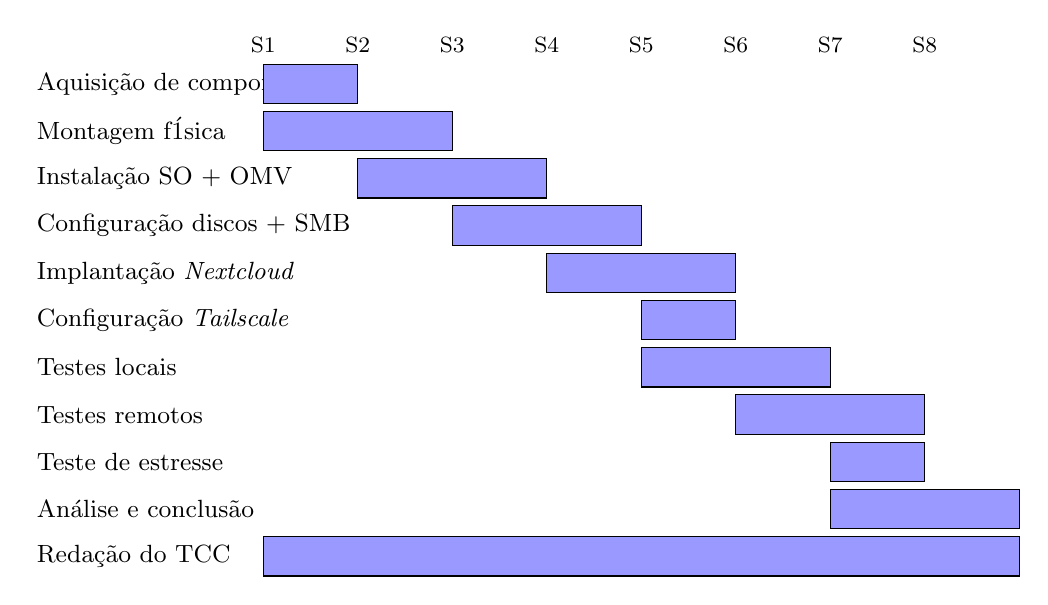
\begin{tikzpicture}[x=1.2cm]
        \tikzstyle{task} = [rectangle, draw, minimum height=0.5cm]

        \foreach \i/\nome in {
            0/{Aquisição de componentes},
            1/{Montagem física},
            2/{Instalação SO + OMV},
            3/{Configuração discos + SMB},
            4/{Implantação \textit{Nextcloud}},
            5/{Configuração \textit{Tailscale}},
            6/{Testes locais},
            7/{Testes remotos},
            8/{Teste de estresse},
            9/{Análise e conclusão},
            10/{Redação do TCC}
        } {
            \node[anchor=west] at (0, -\i*0.6) {\small \nome};
        }

        \draw[fill=blue!40] (2.5, -0*0.6-0.25) rectangle (3.5, -0*0.6+0.25);
        \draw[fill=blue!40] (2.5, -1*0.6-0.25) rectangle (4.5, -1*0.6+0.25);
        \draw[fill=blue!40] (3.5, -2*0.6-0.25) rectangle (5.5, -2*0.6+0.25);
        \draw[fill=blue!40] (4.5, -3*0.6-0.25) rectangle (6.5, -3*0.6+0.25);
        \draw[fill=blue!40] (5.5, -4*0.6-0.25) rectangle (7.5, -4*0.6+0.25);
        \draw[fill=blue!40] (6.5, -5*0.6-0.25) rectangle (7.5, -5*0.6+0.25);
        \draw[fill=blue!40] (6.5, -6*0.6-0.25) rectangle (8.5, -6*0.6+0.25);
        \draw[fill=blue!40] (7.5, -7*0.6-0.25) rectangle (9.5, -7*0.6+0.25);
        \draw[fill=blue!40] (8.5, -8*0.6-0.25) rectangle (9.5, -8*0.6+0.25);
        \draw[fill=blue!40] (8.5, -9*0.6-0.25) rectangle (10.5, -9*0.6+0.25);
        \draw[fill=blue!40] (2.5, -10*0.6-0.25) rectangle (10.5, -10*0.6+0.25);

        \foreach \s in {1,...,8} {
            \node at (\s*1+1.5, 0.5) {\footnotesize S\s};
        }
    \end{tikzpicture}
    \fonteautoria
\end{figure}

As atividades descritas contemplam o escopo completo do TCC, desde a preparação do ambiente experimental até a consolidação dos resultados no texto final. A redação do trabalho ocorre paralelamente às demais atividades, permitindo que cada etapa seja documentada à medida que é executada.
